\documentclass[conference]{IEEEtran}
\usepackage{graphicx,psfrag,epsfig,epsf,latexsym,hhline,amsmath,amssymb,multirow}
\usepackage[usenames,dvipsnames]{pstricks}
\usepackage{pst-plot}
\usepackage{pstricks-add}
\IEEEoverridecommandlockouts
\usepackage{color}
\usepackage{stmaryrd}
\interdisplaylinepenalty=2500
\usepackage{graphicx}
\usepackage{amsthm}
\usepackage{footnote}

\usepackage{blindtext}
\usepackage{etoolbox}
\graphicspath{ {figures:} }

\usepackage{tikz}
\usepackage{pgfplots}
\usepgflibrary{shapes}
\usetikzlibrary{arrows,shapes,chains,matrix,positioning,scopes,patterns	}
\pgfplotsset{compat=newest}
\pgfplotsset{plot coordinates/math parser=false}

%\usepackage{setspace}
%\doublespacing

\newlength\figureheight 
\newlength\figurewidth

\newcommand{\mc}[1]{\mathcal{#1}}
\newcommand{\ms}[1]{\mathscr{#1}}
\newcommand{\mbb}[1]{\mathbb{#1}}
\newcommand{\mbf}[1]{\mathbf{#1}}
\newcommand{\tit}[1]{\textit{#1}}
\newcommand{\tbf}[1]{\textbf{#1}}
\newcommand{\tsc}[1]{\textsc{#1}}

\newcommand{\defeq}{\triangleq}
\newcommand{\coleq}{\mathrel{\mathop:}=}
\newcommand{\Pp}{\mathbb{P}}
\newcommand{\E}{\mathbb{E}}
\newcommand{\N}{\mathbb{N}}
\newcommand{\Z}{\mathbb{Z}}
\newcommand{\Zp}{\mathbb{Z}_{+}}
\newcommand{\R}{\mathbb{R}}
\newcommand{\Rp}{\R_{+}}
\newcommand{\g}{\mathbf{g}_}
\newcommand{\cp}{\times}
\newcommand{\Lmb}{\Lambda}
\newcommand{\lmb}{\lambda}
\newcommand{\tx}[1]{\text{#1}}

\newcommand{\Q}{\mathbb{Q}}
\newcommand{\F}{\mathbb{F}}
\newcommand{\Zw}{\mathbb{Z}[\omega]}
\newcommand{\Zi}{\mathbb{Z}[i]}
\newcommand{\C}{\mathcal{C}}

\newcommand{\abs}[1]{\lvert{#1}\rvert}
\newcommand{\card}[1]{\abs{#1}}
\newcommand{\norm}[1]{\lVert{#1}\rVert}
\newcommand{\iid}{i.\@i.\@d.\ }

\newcommand{\ceil}[1]{\lceil{#1}\rceil}
\newcommand{\floor}[1]{\lfloor{#1}\rfloor}

\DeclareMathOperator*{\argmax}{arg\,max}
\DeclareMathOperator*{\argmin}{arg\,min}

\theoremstyle{definition}\newtheorem{lemma}{Lemma}
\theoremstyle{definition}\newtheorem{proposition}[lemma]{Proposition}
\theoremstyle{definition}\newtheorem{theorem}[lemma]{Theorem}
\theoremstyle{definition}\newtheorem{corollary}[lemma]{Corollary}
\newtheorem{definition}[lemma]{Definition}
\newtheorem{Example}[lemma]{Example}
\newtheorem{Remark}[lemma]{Remark}
\newtheorem*{Discussion}{Discussion}
%\newtheorem{example}[theorem]{Example}



\newcommand{\ind}{{\rm 1\hspace*{-0.4ex}\rule{0.1ex}{1.52ex}\hspace*{0.2ex}}}
\newcommand{\dbar}[1]{\bar{\bar{#1}}}
\newcommand{\T}{\msf{T}}
\newcommand{\dotleq}{\mathrel{\dot{\leq}}}
\newcommand{\dotgeq}{\mathrel{\dot{\geq}}}
\newcommand{\dotl}{\mathrel{\dot{<}}}
\newcommand{\dotg}{\mathrel{\dot{>}}}
\newcommand{\from}{\colon}

\DeclareMathOperator{\rank}{rank}
\DeclareMathOperator{\tr}{tr}
\DeclareMathOperator{\cl}{cl}
\DeclareMathOperator{\diag}{diag}
\DeclareMathOperator{\conv}{conv}
\DeclareMathOperator{\Bernoulli}{Bernoulli}
\DeclareMathOperator{\Ei}{Ei}
\DeclareMathOperator{\OR}{OR}
\DeclareMathOperator{\Geom}{Geom}
\DeclareMathOperator{\var}{var}

\begin{document}
\title{Multilevel Lattices based on Spatially-Coupled LDPC Codes with Applications}
\author{Avinash Vem, Yu-Chih Huang, Krishna R. Narayanan, Henry D. Pfister,\thanks{The material in this work was funded in parts by the National Science Foundation under Grants CCF 13202924 and CCF 1302616.
}\\
Department of Electrical and Computer Engineering \\
Texas A\&M University\\
{\tt\small {\{avinash.iitm42@tamu.edu, jerry.yc.huang@gmail.com, krn@ece.tamu.edu, hpfister@tamu.edu\}} }}

\maketitle

\begin{abstract}
We propose a class of lattices constructed using Construction D where the underlying linear codes are nested binary spatially-coupled low-density parity-check codes (SC-LDPC) codes with uniform left and right degrees. By leveraging recent results on the optimality of spatially-coupled codes for binary input memoryless channels and Forney {\em et al.}'s earlier results on the optimality of construction D, we show that the proposed lattices achieve the Poltyrev limit under multistage belief propagation decoding. Lattice codes constructed from these lattices are shown to provide excellent performance for the three user symmetric interference channel. They can also be naturally used in applications such as integer-forcing and compute-and-forward.
\end{abstract}


\section{Introduction}
Lattice codes obtained from nested lattices have been shown to be optimal coding solutions to several problems in information theory \cite{erez05}. In most of these cases, the underlying lattices are constructed using Construction A and it has been shown that such lattices are simultaneously good for shaping (Roger's good) and for channel coding (Poltyrev good) \cite{erez05}. There are two important drawbacks in using optimal lattices constructed using Construction A. On the theoretical side, the use of non-binary codes makes it difficult to prove the optimality of these lattices and lattice codes under practical decoding algorithms such as belief propagation (BP) decoding and so far, we are not aware of any results showing the optimality of Construction A lattices under BP decoding. On the practical side, optimal lattices constructed from Construction A typically require the underlying linear codes to work over large fields and hence, result in formidable decoding complexity, even with BP decoding.

In this paper, we propose a class of lattices constructed using Construction D \cite{BarnesSloane83} where the underlying linear codes are nested binary spatially-coupled low-density parity-check codes (SC-LDPC) codes with uniform left and right degrees. By using the result that regular SC-LDPC codes can universally achieve capacity under BP decoding for the class of binary memoryless symmetric (BMS) channels  \cite{kudekaruniversal,kumar2012proof} and by leveraging Forney {\em et al}'s result \cite{forney2000}, we show that the proposed lattices allow us to achieve the Poltyrev
limit under multistage BP decoding. We refer to the proposed lattices as SC-LDPC lattices. Density evolution thresholds show that the proposed SC-LDPC lattices can approach the Poltyrev limit to within 0.1 dB under multistage BP decoding. Very recently, binary polar codes have been used in conjunction with Construction D to obtain Poltyrev-good lattices in \cite{YanLingWu13}. The focus of this paper is on the use of SC-LDPC codes. Both these approaches have merits and disadvantages, and a detailed comparison needs to be undertaken as part of future work. It should also be noted that in \cite{sadeghi06}, construction D' lattices using LDPC codes have been proposed along with a joint message passing decoding algorithm.

We then construct lattice codes from this class of lattices using hypercube shaping and we apply them to the symmetric $k$-user interference channel \cite{sridharan2008capacity}. We show that for channel gains which are within 0.39~dB from the very strong interference regime, the desired user can be decoded at signal-to-noise ratios within 1.53~dB from the Shannon limit. For practical check degrees, simulation results with BP decoding show a gap of about 2.6~dB from the Shannon limit. This class of lattice codes can also be applied to Integer-forcing or compute-and-forward in the multiple access stage \cite{nazer2011CF}.

%Recently, it has been pointed out in \cite{Estela13} that there is a natural connection between lattices generated by Construction D (or Construction D$^\prime$) and the interference alignment scheme in \cite{jafar10}. Thus, one can directly implement interference alignment by replacing the
%Barnes-Wall lattices in \cite{Estela13} by our proposed SC-LDPC lattices. Simulation results show that this replacement
%leads us to a significant gain in terms of bit error probability.

Throughout the rest of the paper, vectors and matrices are written in lowercase boldface and uppercase boldface, respectively.

\section{Background}
\label{Section:Background}
\subsection{Lattices and Poltyrev Limit}
Consider a lattice $\Lmb$ with a fundamental volume $V(\Lmb)$. Let us assume that some $\mathbf{\boldsymbol\lambda}\in\Lmb$ is transmitted through an additive white Gaussian noise (AWGN) channel of variance $\sigma^{2}$ and denote the noise
vector by $\mathbf{z}$. Let us denote the probability of decoding error, conditioned on codeword $\boldsymbol\lambda 	\in\Lambda$ being
transmitted as $P(\mathbf{\boldsymbol\lambda},\sigma^{2})$ which is defined as
\begin{align*}
 P(\boldsymbol\lambda,\sigma^{2}):=\Pr(d(\boldsymbol\lambda,\boldsymbol\lambda+\mathbf{z})\geq d(\boldsymbol\lambda',\boldsymbol\lambda'+\mathbf{z})) \text{ for some } \boldsymbol\lambda' \in\Lmb,
\end{align*}
where $d(\mathbf{x},\mathbf{y})$ is the Euclidean distance between $\mathbf{x}$ and $\mathbf{y}$. For an infinite lattice $\Lmb$, $P(\boldsymbol\lambda,\sigma^{2})$ is independent of $\boldsymbol\lambda$ and hence the average probability of decoding error for the lattice  $P(\Lmb,\sigma^{2})$ is the same as $P(\boldsymbol\lambda,\sigma^{2})$ for any $\boldsymbol\lambda$.
%Let $Cb(a)$ denote the cube of side $a$ centered at
%origin. We shall  define, $ P(\Lmb,\sigma^{2})$, average probability of decoding error for $\boldsymbol\lambda$, as
%\begin{align*}
% p(\Lmb,\sigma^{2})=\lim_{a\rightarrow \infty}|\Lmb\cap Cb(a)|^{-1}\sum_{\boldsymbol\lambda\in \Lmb\cap Cb(a)}p(\boldsymbol\lambda,\sigma^{2}).
%\end{align*}
The volume-to-noise ratio (VNR), $\alpha^{2}(\Lmb,\sigma^{2})$,
of an $n$-dimensional lattice $\Lmb$ is given by $\alpha^{2}(\Lmb,\sigma^{2})=\frac{V(\Lmb)^{2/n}}{2\pi e\sigma^{2}}$.
Poltyrev in \cite{poltyrev94} showed that for any VNR $>1$ there exists a sequence of lattices for which $P(\Lmb,\sigma^{2}) \rightarrow 0$ as $n \rightarrow \infty$. We shall call such a sequence of lattices as being Poltyrev-good.

\subsection{Construction D and its Goodness}
In this section we briefly describe Construction D lattices \cite{BarnesSloane83} \cite{conway1999sphere} and then recall Forney {\em et al}'s result on the existence of Poltyrev-good lattices based on this construction \cite{forney2000}.

For any lattice $\Lmb$, a sub-lattice $\Lmb^\prime\subset \Lmb$ induces a coset decomposition ($\Lmb/\Lmb^\prime$)
of $\Lmb$. i.e., it partitions $\Lmb$ into equivalence groups modulo $\Lmb^\prime$. We call this a lattice partition.
Construction D and D' are multistage constructions of lattices that are based on such a partition chain and a sequence of nested
linear codes $\{\mathcal{C}_{l},1\leq l\leq r\}$ where each code $\mathcal{C}_{l}$ is of length $n$ over $\mathbb{F}_q$, where $\mathbb{F}_q \cong \Lmb_{l-1}/\Lmb_{l}$.
%For more details we refer to \cite{forney2000}.
%Construction D and Construction D$^{\prime}$ are based on such nested sequence of linear codes.
For a detailed description we refer to \cite{conway1999sphere}. In our work we use a one-dimensional lattice partition chain
 $\Lmb_{0}/\Lmb_{1}/\cdots /\Lmb_{r}$, where $\Lmb_{i}=2^{i}\Z$. Then
$\Lmb_{i-1}/\Lmb_{i}\cong \mathbb{F}_{2}$ for all $i$. Let $\mathcal{C}_{i}$ be a $(n,k_i)$ binary code spanned by the
set of linearly independent binary $n$-tuples $\{\mathbf{g}_1,\mathbf{g}_2,\ldots,\mathbf{g}_{k_i}\}$ where $k_{1}\leq k_{2}\leq \cdots \leq k_{r}$. Using nested binary linear codes
$\{\mathcal{C}_{j},1\leq j\leq r\}$, a multistage Construction-D type lattice is defined as follows:
\begin{align}\label{Eqn:ConstrD}
 \Lmb=\biggl\{2^{r}\Z^{n}+\sum_{1\leq j\leq r}\sum_{1\leq i\leq k_{j}}\alpha_{ji}2^{j-1}\mathbf{g}_i|\alpha_{ji}\in\{0,1\}\biggr\},
\end{align}
where ``$+$" denotes addition in $\R^{n}$. The VNR of a Construction D lattice described above is given by
\begin{equation}
    \alpha^{2}(\Lmb,\sigma^{2})=\frac{2^{2(r-\sum_{i=1}^{r}k_{i}/n)}}{2\pi e\sigma^{2}}.
\end{equation}
%\begin{equation}
%    10\log_{10}\alpha^{2}(\Lmb,\sigma^{2})=10\log_{10}\left(\frac{2^{2(r-\sum_{1}^{r}k_{i})}}{2\pi e\sigma^{2}}\right) \text{~~dB}.
%\end{equation}
Let $\boldsymbol\lambda\in\Lmb$, where $\Lmb$ is as defined in \eqref{Eqn:ConstrD}, be transmitted through an AWGN channel and
$\mathbf{y}=\boldsymbol\lambda+\mathbf{z}$ is received where $\mathbf{z}\sim\mathcal{N}(0,\sigma^{2}\cdot \mathbf{I})$. Let $\hat{\mathbf{y}}_{0}=\mathbf{y}$. The multistage decoder for decoding $\boldsymbol\lambda\in \Lambda$ uses the following steps.
\begin{itemize}
\item \textbf{Step 1}: At stage $j, $ $1\leq j\leq r$, $\hat{\mathbf{y}}_{j-1}\mod 2$ is decoded to a codeword  $\hat{\mathbf{x}}_{j}\in \mathcal{C}_{j}$ and the corresponding information
bits  $\{\hat{\alpha}_{j1},\hat{\alpha}_{j2},\cdots, \hat{\alpha}_{jk_{j}}\}\in \{0,1\}^{k_{j}}$ that generate $\hat{\mathbf{x}}_{j}$,
are computed.
\item \textbf{Step 2}: Compute $\hat{\mathbf{y}}_{j}= \frac{1}{2} \cdot(\hat{\mathbf{y}}_{j-1}-\sum_{1\leq i\leq k_{j}}\hat{\alpha}_{ji}\mathbf{g}_i)$. Repeat \textbf{Step 2}.
\item \textbf{Step 3}: At $(r+1)^{\text{th}}$ stage of decoding, $\hat{\mathbf{y}}_{r}$ is decoded to the closest $\mathbf{q}\in\Z^{n}$.
\item \textbf{Output}: The decoded lattice point $\hat{\mathbf{\boldsymbol\lambda}}\in\Lmb$ is given by
\begin{align}
    \hat{\mathbf{\boldsymbol\lambda}}=2^{r}\mathbf{q}+\sum_{1\leq j\leq r}\sum_{1\leq i\leq k_{j}}\hat{\alpha}_{ji}2^{j-1}\mathbf{g}_i.
\end{align}
\end{itemize}

At the $j^{\text{th}}$ stage of decoding, conditioned on successful decoding in previous stages, the input to the decoder has the form
\begin{align}
\hat{\mathbf{y}}_{j-1} \hspace{-8pt}\mod 2%&=\frac{1}{2}\left(\hat{\mathbf{y}}_{j-2}-\sum_{1\leq i\leq k_{j-1}}\alpha_{(j-1)i}\mathbf{g}_i\right)\hspace{-8pt}\mod 2\notag\\
%&=\left( \frac{1}{2^{j-1}}\hat{\mathbf{y}}_{0}-\sum_{1\leq p< j}2^{p-j}\sum_{1\leq i\leq k_{p}}\alpha_{pi}\mathbf{g}_i \right) \hspace{-8pt}\mod 2\notag\\
&=\frac{1}{2^{j-1}}\left( \mathbf{y}-\sum_{1\leq p< j}\sum_{1\leq i\leq k_{p}}2^{p-1}\alpha_{pi}\mathbf{g}_i \right) \hspace{-8pt}\mod 2\notag\\
&=\left(\sum_{i=1}^{k_{j}}\alpha_{ji}\mathbf{g}_i \right) \hspace{-8pt}\mod 2 + \left( 2^{-(j-1)}\mathbf{z} \right) \hspace{-8pt}\mod 2\notag\\
&=\mathbf{x}_{j}+2^{-(j-1)}\mathbf{z} \hspace{-8pt}\mod 2,
\label{Eqn:Mod2Channel}
\end{align}
where $\mathbf{x}_{j}\in\mathcal{C}_{j}$. We call the channel defined in \eqref{Eqn:Mod2Channel} as an additive mod-2 Gaussian noise (AMGN) channel \cite{forney2000} and denote the capacity for this channel as  $C(\Z/2\Z,2^{-2(j-1)}\sigma^{2})$ which is shown to be equal to $C(2^{j-1}\Z/2^{j}\Z,\sigma^{2})$\cite{forney2000}.

\begin{theorem}[Forney \textit{et al.} \cite{forney2000}]
For an AWGN channel with noise variance per dimension $\sigma^{2}$, there exists a sequence of Construction D lattices $\Lmb$ based on a chain of two-way one-dimensional lattice partitions and $r$ nested random binary linear codes $\mathcal{C}_{1}\subseteq \mathcal{C}_{2}\subseteq\cdots \subseteq \mathcal{C}_{r}$ that is Poltyrev-good.
\end{theorem}
\begin{remark}\label{rmk:Forney_proof}
    Note that in \cite{forney2000}, it was shown that if for each level $j\in\{1,\ldots,r\}$, the linear code $\mathcal{C}_{j}$ at that level achieves the capacity $C(2^{j-1}\Z/2^{j}\Z,\sigma^{2})$ then the Construction
    D lattice thus constructed is Poltyrev-good.
\end{remark}

\section{Proposed SC-LDPC Lattices}\label{Sec:SCLDPC}
%These nested linear codes will then be used for constructing the proposed SC-LDPC lattices. We then show the existence of a sequence of the proposed lattices that is Poltyrev-good and provide simulation results which verify our theoretical results.

Construction of lattices based on Construction D using a SC-LDPC code at each level requires the SC-LDPC codes to be nested. In this section, we first construct such a sequence of nested linear codes based on ensembles of SC-LDPC codes such that each of the code ensembles in the nested construction is capacity achieving. For ease of exposition, we restrict our description to $r=2$.
%
% The familiar construction of Tanner graphs for these codes \cite{KudekarUrbanke11} involves totally random permutation of edges between systems
% within some coupling width. In this construction, removal of a fraction of check nodes results in a SC-LDPC supercode, but the
% regularity of the degree profile is lost and the analysis of resulting code is very complicated. For this purpose
%we propose a construction where the random permutation of edges have some structure to it (i.e., not totally random) where in
%deletion of a fraction of check nodes results again in a regular SC-LDPC code.

\subsection{Construction}
Given the rates of $\mc{C}_1$ and $\mc{C}_2$ as $r_{1}$ and $r_{2}$, respectively, with $r_{1}<r_{2}$, we construct
the nested SC-LDPC code ensemble parameterized by $(L,w)$ where $L$ is the
number of independent LDPC systems coupled and $w$ is the coupling width whose design rates tend to $r_{1}$ and $r_{2}$, respectively,
 in the limit of $w,L\rightarrow \infty$. Choose $d_{c}\in\Z$ large enough such that there exists $d_{v}^{1},d_{v}^{2}\geq 3\in\Z$ and
\begin{align*}
    1-\frac{d_{v}^{1}}{d_{c}}>r_{1}-\epsilon\text{  and } 1-\frac{d_{v}^{2}}{d_{c}}>r_{2}-\epsilon.
\end{align*}

Our approach is to first construct a rate $r_{1}$ regular LDPC code ensemble and then obtain the rate $r_{2}$ ensemble by removing a fraction of the parity checks and the edges incident on these checks in a way that both the ensembles are regular SC-LDPC code ensembles which are universally capacity achieving. The ensemble described in \cite{KudekarUrbanke11} is not directly amenable to this approach of deriving the higher rate code, since removing a fraction of the checks from this ensemble does not result in a regular SC-LDPC code ensemble. Therefore, our approach is to use the following multi-edge type construction.

We place $Md_{c}$ variable nodes at positions $[1,L]$, $L\in\N$ and $Md_{v}^{1}$ check nodes at positions $[1,L+w-1]$, where $w\in \N$ is the coupling width. At each position divide the $Md_{v}^{1}$ check nodes into $d_{v}^{1}$ groups where each group contains $M$ check nodes. At any position we refer to all check nodes belonging to $k^{th}$ group as of type $\mc{T}_{k}$ i.e.,  at each position there are $d_{v}^{1}$ types of check nodes with $M$ check nodes of each type. Similarly, for each variable node, we classify the $d_{v}^{1}$ edges into types where $k^{\text{th}}$ edge is referred to as type $\mc{E}_{k}$ and hence, at each position there are $Md_{c}$ edges of each type. For all $i\in\{1,2,\ldots,L\}$ and $k\in\{1,2,\ldots ,d_{v}^{1}\}$, connections for $Md_{c}$ edges of type $\mc{E}_{k}$ of the variable nodes at position $i$ are chosen uniformly and independently from all type $\mc{T}_{k}$ check nodes in the range $\{i,\ldots , i+w-1\}$. This results in a Tanner graph in which every variable node has exactly one edge connected to type $\mc{T}_{k}$ check node for all $k\in \{1,2,\ldots , d_{v}^{1}\}$. We call such graph as a \textit{check-uniform connected graph}.

From such a Tanner graph, removal of all check nodes of a particular type, say $\mc{T}_{1}$, results in a variable node degree of $d_{v}^{1}-1$.  One can see that
removal of all check nodes of types $\mc{T}_{1},\mc{T}_{2},\ldots, \mc{T}_{d_{v}^{1}-d_{v}^{2}} $ from the original Tanner graph results in a $(d_{v}^{2},d_{C})$ SC-LDPC graph that is a sub-graph of the original graph.
%The proposed construction slightly differs from the original construction in \cite{KudekarUrbanke11} and
We call the proposed construction as \textit{check-uniform} SC-LDPC (CU-SC-LDPC) ensemble of codes. Thus one can obtain a sequence of nested regular SC-LDPC codes for any non-increasing sequence $d_{v}^{1}\geq d_{v}^{2}\geq\cdots \geq d_{v}^{r}$. 
We refer to such a nested ensemble as $(d_{v}^{1},\ldots ,d_{v}^{r},d_{c})$ CU-SC-LDPC ensemble.
%by removing repeatedly performing the above operation. 
 \begin{figure}[h!]
\centering
\scalebox{1}[0.78]{\input{./figures/Basegraph.tex}}
\caption{Example of a $(3,6)$ CU-SP-LDPC code for $L=3$, $w=2$, $M=1$. Removal of all the type $\mc{T}_{1}$ check nodes i.e the shaded ones, results in a $(2,6)$ CU-SC-LDPC code.}
\label{Basegraph}
\end{figure}

%  \begin{figure}[h!]
%\centering
%%\begin{document}
%\usepackage{tikz,pgfplots}
\usetikzlibrary{arrows,shapes,chains,matrix,positioning,scopes,patterns,fit}
\usetikzlibrary{decorations.markings,decorations.pathmorphing,backgrounds}

\usepgfplotslibrary{groupplots}
\usetikzlibrary{external}

\usepackage{graphicx,psfrag,epsfig,epsf,latexsym,hhline,amsmath,amssymb,multirow}
\usepackage{pst-plot}
\usepackage{color}
\usepackage{stmaryrd}
\usepackage{makecell}
\usepackage{fontenc}
\usepackage{footnote}
\usepackage{blindtext}
\usepackage{etoolbox}
\usepackage{stmaryrd}
\usepackage{subfigure}
\usepackage{xcolor}

\pgfplotsset{compat=newest}
\pgfplotsset{plot coordinates/math parser=false}

\interdisplaylinepenalty=2500
%\newlength\figureheight 
\newlength\figurewidth

\newcommand{\mc}[1]{\mathcal{#1}}
\newcommand{\ms}[1]{\mathscr{#1}}
\newcommand{\mbb}[1]{\mathbb{#1}}
\newcommand{\mbf}[1]{\mathbf{#1}}
\newcommand{\tit}[1]{\textit{#1}}
\newcommand{\tbf}[1]{\textbf{#1}}
\newcommand{\tsc}[1]{\textsc{#1}}

\newcommand{\defeq}{\triangleq}
\newcommand{\coleq}{\mathrel{\mathop:}=}
\newcommand{\Pp}{\mathbb{P}}
\newcommand{\E}{\mathbb{E}}
\newcommand{\N}{\mathbb{N}}
\newcommand{\Z}{\mathbb{Z}}
\newcommand{\Zp}{\mathbb{Z}_{+}}
\newcommand{\R}{\mathbb{R}}
\newcommand{\Rp}{\R_{+}}
\newcommand{\g}{\mathbf{g}_}
\newcommand{\cp}{\times}
\newcommand{\Lmb}{\Lambda}
\newcommand{\lmb}{\lambda}
\newcommand{\tx}[1]{\text{#1}}

\newcommand{\Q}{\mathbb{Q}}
\newcommand{\F}{\mathbb{F}}
\newcommand{\Zw}{\mathbb{Z}[\omega]}
\newcommand{\Zi}{\mathbb{Z}[i]}
\newcommand{\C}{\mathcal{C}}

\newcommand{\abs}[1]{\lvert{#1}\rvert}
\newcommand{\card}[1]{\abs{#1}}
\newcommand{\norm}[1]{\lVert{#1}\rVert}
\newcommand{\iid}{i.\@i.\@d.\ }

\newcommand{\ceil}[1]{\lceil{#1}\rceil}
\newcommand{\floor}[1]{\lfloor{#1}\rfloor}

\DeclareMathOperator*{\argmax}{arg\,max}
\DeclareMathOperator*{\argmin}{arg\,min}

\theoremstyle{definition}\newtheorem{lemma}{Lemma}
\theoremstyle{definition}\newtheorem{proposition}[lemma]{Proposition}
\theoremstyle{definition}\newtheorem{theorem}[lemma]{Theorem}
\theoremstyle{definition}\newtheorem{corollary}[lemma]{Corollary}
\newtheorem{definition}[lemma]{Definition}
\newtheorem{Example}[lemma]{Example}
\newtheorem{Remark}[lemma]{Remark}
\newtheorem*{Discussion}{Discussion}
%\newtheorem{example}[theorem]{Example}



\newcommand{\ind}{{\rm 1\hspace*{-0.4ex}\rule{0.1ex}{1.52ex}\hspace*{0.2ex}}}
\newcommand{\dbar}[1]{\bar{\bar{#1}}}
\newcommand{\T}{\msf{T}}
\newcommand{\dotleq}{\mathrel{\dot{\leq}}}
\newcommand{\dotgeq}{\mathrel{\dot{\geq}}}
\newcommand{\dotl}{\mathrel{\dot{<}}}
\newcommand{\dotg}{\mathrel{\dot{>}}}
\newcommand{\from}{\colon}

\DeclareMathOperator{\rank}{rank}
\DeclareMathOperator{\tr}{tr}
\DeclareMathOperator{\cl}{cl}
\DeclareMathOperator{\diag}{diag}
\DeclareMathOperator{\conv}{conv}
\DeclareMathOperator{\Bernoulli}{Bernoulli}
\DeclareMathOperator{\Ei}{Ei}
\DeclareMathOperator{\OR}{OR}
\DeclareMathOperator{\Geom}{Geom}
\DeclareMathOperator{\var}{var}
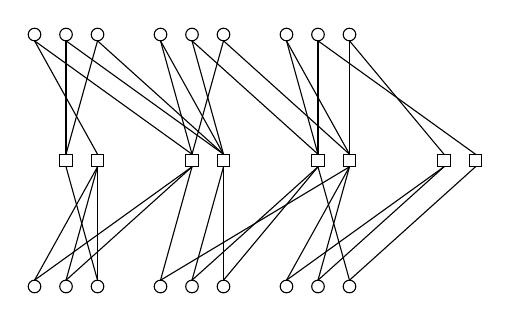
\begin{tikzpicture}[scale=0.8]

   \draw [black] (0,2) circle (0.1);  \draw [black] (0,-2) circle (0.1);
\draw [black] (0.6,0.1) rectangle (0.4,-0.1);  	\draw [black] (0.5,2) circle (0.1);  \draw [black] (0.5,-2) circle (0.1);
\draw [black] (1.1,0.1) rectangle (0.9,-0.1);     \draw [black] (1,2) circle (0.1);  \draw [black] (1,-2) circle (0.1);
  \draw (0,1.9) -- (2.5,0.1); \draw (0,1.9) -- (1,0.1);
\draw (0.5,1.9) -- (0.5,0.1); \draw (0.5,1.9) -- (3,0.1);
 \draw (1,1.9) -- (0.5,0.1); \draw (1,1.9) -- (3,0.1);

 \draw (0,-1.9) -- (2.5,-0.1); \draw (0,-1.9) -- (1,-0.1);
  \draw (0.5,-1.9) -- (2.5,-0.1); \draw (0.5,-1.9) -- (1,-0.1);
  \draw (1,-1.9) -- (0.5,-0.1); \draw (1,-1.9) -- (1,-0.1);

 \draw [black] (2,2) circle (0.1);  \draw [black] (2,-2) circle (0.1);
\draw [black] (2.6,0.1) rectangle (2.4,-0.1);  	\draw [black] (2.5,2) circle (0.1);  \draw [black] (2.5,-2) circle (0.1);
\draw [black] (3.1,0.1) rectangle (2.9,-0.1);  	\draw [black] (3,2) circle (0.1);  \draw [black] (3,-2) circle (0.1);
 \draw (2,1.9) -- (2.5,0.1); \draw (2,1.9) -- (3,0.1);
  \draw (2.5,1.9) -- (4.5,0.1); \draw (2.5,1.9) -- (3,0.1);
\draw (3,1.9) -- (2.5,0.1); \draw (3,1.9) -- (5,0.1);

 \draw (2,-1.9) -- (2.5,-0.1); \draw (2,-1.9) -- (5,-0.1);
 \draw (2.5,-1.9) -- (4.5,-0.1); \draw (2.5,-1.9) -- (3,-0.1);
  \draw (3,-1.9) -- (4.5,-0.1); \draw (3,-1.9) -- (3,-0.1);

\draw [black] (4,2) circle (0.1);  \draw [black] (4,-2) circle (0.1);
\draw [black] (4.6,0.1) rectangle (4.4,-0.1);      \draw [black] (4.5,2) circle (0.1);  \draw [black] (4.5,-2) circle (0.1);
\draw [black] (5.1,0.1) rectangle (4.9,-0.1);    \draw [black] (5,2) circle (0.1);  \draw [black] (5,-2) circle (0.1);
  \draw (4,1.9) -- (4.5,0.1); \draw (4,1.9) -- (5,0.1);
 \draw (4.5,1.9) -- (4.5,0.1); \draw (4.5,1.9) -- (7,0.1);
  \draw (5,1.9) -- (6.5,0.1); \draw (5,1.9) -- (5,0.1);

\draw (4,-1.9) -- (6.5,-0.1); \draw (4,-1.9) -- (5,-0.1);
 \draw (4.5,-1.9) -- (6.5,-0.1); \draw (4.5,-1.9) -- (5,-0.1);
 \draw (5,-1.9) -- (4.5,-0.1); \draw (5,-1.9) -- (7,-0.1);


\draw [black] (6.6,0.1) rectangle (6.4,-0.1);   %\draw [black] (13,2) circle (0.1);  \draw [black] (13,-2) circle (0.1);
\draw [black] (7.1,0.1) rectangle (6.9,-0.1);   %\draw [black] (14,2) circle (0.1);  \draw [black] (14,-2) circle (0.1);

 \end{tikzpicture}

%\end{document}
%\caption{Base Graph for $(2,6)$, $\Gamma_{2}$ derived from the base graph of  ($3,6$), $\Gamma_{1}$, by removing all type $•\mc{T}_{c_{1}}$ check nodes, for parameters $L=3$, $w=2,M=1$.}
%\label{BaseGraph_sup}
%\end{figure}

It can be seen that for a sequence of nested binary linear codes $\C_{1}\subseteq \mathcal{C}_{2}\subseteq\ldots \subseteq\mathcal{C}_{r}$ there exists nested generator matrices for these codes and hence, we can use Construction D described in \eqref{Eqn:ConstrD} with the proposed CU-SC-LDPC codes. We refer to a lattice thus constructed as a nested SC-LDPC lattice.

%Since Construction D works with generator matrices of nested linear codes, we have to obtain nested generator matrices from the proposed nested CU-SC-LDPC codes. In the following lemma (stated without proof due to page length restrictions), we show the existence of such nested generator matrices for any set of nested binary linear codes.
%\begin{lemma}\label{lemma:nested_G}
%    Given nested binary linear codes $\C_{1}\subseteq \mathcal{C}_{2},\ldots, \subseteq\mathcal{C}_{r}$ there exists nested generator matrices for these codes.
%\end{lemma}
%%\begin{IEEEproof}
%%It suffices to consider the case having only two levels. For $\mathcal{C}_{1}$ there exists set of linearly independent binary vectors
%%$\mathbf{G}_{1}=\{\mathbf{g}_1,\mathbf{g}_2,\ldots, \mathbf{g}_{k_1}\}$ that span $\mathcal{C}_{1}$ where $k_{1}=$dim$(\mathcal{C}_{1})$.
%%Denote $\mathbf{Z}_{i}=\{\mathbf{G}_{1},\mathbf{g}_{k_{1}+1},\mathbf{g}_{k_{1}+2}, \ldots, \mathbf{g}_{k_{1}+i-1}\}$ and $Y_{i}=\mathcal{C}_{2}\setminus$
%%span$(\mathbf{Z}_{i})$ for $i=1,2, \ldots, k_{2}-k_{1}$. Note that for any $\mathbf{x}\in Y_{i}$, $\mathbf{x}$ is linearly independent with $\mathbf{Z}_{i}$ and hence
%%$\mathbf{Z}_{i+1}=\{\mathbf{Z}_{i},\mathbf{g}_{k_{1}+i}\}$ forms a linearly independent set where $\mathbf{g}_{k_{1}+i}=\mathbf{x}$. This recursive procedure gives us a basis $\mathbf{G}_{2}$ for $\mathcal{C}_{2}$. Thus the existence of the generator matrices for nested binary linear codes is shown.
%%\end{IEEEproof}
%From the above Lemma~\ref{lemma:nested_G}, given nested CU-SC-LDPC codes $\mathcal{C}_{1}\subset \mathcal{C}_{2}\ldots \subset\mathcal{C}_{r}$,
%one can find a corresponding sequence of nested sets of generator vectors $\mathbf{G}_{1}\subset \mathbf{G}_{2}
%\subset \ldots \subset\mathbf{G}_{r}$ and hence can use Construction D described in \eqref{Eqn:ConstrD} with the proposed CU-SC-LDPC codes. We refer to the lattices thus constructed as the \textit{SC-LDPC lattice}.
\subsection{Poltyrev-Goodness of the Proposed Lattices}
We now show the existence of a sequence of SC-LDPC lattices which is Poltyrev-good under BP decoding. In the following lemmas, we show that the proposed CU-SC-LDPC codes achieve the AMGN channel capacity. We then follow the argument by Forney \textit{et al.} described in Remark~\ref{rmk:Forney_proof} to show the result.

\begin{lemma}\label{lemma:DE_SCLDPC}
For a BMS channel with associated L-density $\mathbf{x}_{\text{BMS}}$, the density evolution (DE) equation for a ($d_{v},d_{c},w,L$) CU-SC-LDPC ensemble is given by
\begin{align}
%x_{i}^{(l)}=\epsilon\left( \frac{1}{w}\sum_{j=0}^{w-1}\left(\frac{1}{w}\sum_{k=0}^{w-1}x_{i+j-k}^{(l-1)}\right)^{d_{r}-1} \right)^{d_{l}-1},
\mathbf{x}_{i}^{(l)}=\mathbf{x}_{\text{BMS}}\circledast\left(\frac{1}{w}\sum_{j=0}^{w-1}\left(\frac{1}{w}\sum_{k=0}^{w-1}\mathbf{x}_{i+j-k}^{(l-1)}\right)^{\boxast d_{c}-1} \right)^{\circledast d_{v}-1},
\label{Eqn:DE_SCLDPC}
\end{align}
where $\mathbf{x}_{i}^{(l)}$ is the average L-density of a variable node at position $i$ in iteration $l$.
\end{lemma}
\begin{IEEEproof}
In the proposed CU-SC-LDPC ensemble, from the perspective of a variable node there are $d_{v}$ types of edges $\mc{E}_{1},\mc{E}_{2},\cdots,\mc{E}_{d_{v}}$. We denote edges of type $\mc{E}_{k}$ that originate from a variable node at position $i$ as $(i,\mc{T}_{k})$ and the L-density of the message emitted by variable nodes along such edge types as $\mathbf{x}_{ik}^{(l)}$ where
 $l$  denotes the iteration. But from the perspective of a check node of any type at position $i$, an edge is randomly
connected to one of the variable nodes located at positions $\{i, i-1,\ldots ,i-w+1\}$.	Hence all the edges connected to check nodes at a certain position are statistically identical and more importantly all check nodes at certain position are statistically identical.
The average L-density of the message emitted by a check node at position $i$ in iteration $l$, denoted by $\mathbf{y}_{i}^{(l)}$, is given by
\begin{align}
\mathbf{y}_{i}^{(l)}=\left(\frac{1}{w}\sum_{j=0}^{w-1}\left(\frac{1}{d_{v}}\sum_{k=0}^{d_{v}}\mathbf{x}_{(i-j)k}^{(l-1)}\right)\right)^{\boxast d_{c}-1}
\label{Eqn:CheckNodeUpdate}
\end{align}
And a variable node update is given by
\begin{align}
\mathbf{x}_{ik}^{(l)}&=\mathbf{x}_{\text{BMS}}\circledast \left(\frac{1}{w}\sum_{j=0}^{w-1}\mathbf{y}_{i+j}^{(l)}\right)^{\circledast d_{v}-1}\label{Eqn:VariableNodeUpdate}\\
\mathbf{x}_{i}^{(l)}&=\frac{1}{d_{v}}\sum_{k=0}^{d_{v}}\mathbf{x}_{ik}^{(l)}\notag
\end{align}
where $\mathbf{x}_{i}^{(l)}$ is the average L-density of the log-likelihood ratio of variable nodes at position $i$.
Combining \eqref{Eqn:CheckNodeUpdate} and \eqref{Eqn:VariableNodeUpdate} and observing that the initialization
is $\mathbf{x}_{i}^{(1)}=\mathbf{x}_{i1}^{(1)}=\mathbf{x}_{i2}^{(1)}=\cdots=\mathbf{x}_{id_{v}}^{(1)}=\mathbf{x}_{\text{BMS}}$ completes the proof.
\end{IEEEproof}

Note that the DE equations for the proposed CU-SC-LDPC ensemble in \eqref{Eqn:DE_SCLDPC} are identical to that of SC-LDPC ensemble proposed in \cite{KudekarUrbanke11,kudekaruniversal}.
%Moreover, DE equations for any BMS channel are merely an extension of the scalar version of DE for a BEC channel to a vector version where the product operation is replaced by convolution in respective domains and sum of scalars replaced by sum of vectors. Therefore for any BMS channel the equivalence of DE for both the ensembles follow.

\begin{lemma}\label{lemma:BMSProof}
For any $\epsilon>0$, there exists a sequence of $(d_{v},d_{c})$ CU-SC-LDPC codes parameterized by ($L,w$) such that the rate $R>C_{\text{AMGN}}-\epsilon$ as $L \rightarrow \infty$, for which the bit error probability under BP decoding $\rightarrow 0$  as $M\rightarrow \infty$, where $C_{\text{AMGN}}$ is the Shannon capacity of the AMGN channel.
\end{lemma}
\begin{IEEEproof}
It has been proved in \cite{kudekaruniversal,kumar2012proof} that over any BMS channel, under BP decoding, any system that satisfies the equation \eqref{Eqn:DE_SCLDPC} achieves capacity as $d_{c},w,L \rightarrow \infty$ (with $\frac{d_{v}}{d_{c}}$ fixed). Hence, using Lemma \ref{lemma:DE_SCLDPC}, it suffices to show that the AMGN channel described in \eqref{Eqn:Mod2Channel} is indeed a BMS channel. This can be seen from the proof in \cite{YanLingWu13}.
%It is clear to see that the AMGN channel has binary input and output lying in an interval of length $2$. Let the input alphabet to the channel be $\{0,1\}$ and without loss of generality let the $\mod 2$ operation produces a output lying in $[-0.5,  1.5]$. Then the conditional PDFs of $\mathbf{y}$ can be written as
%\begin{align}
%f(y|x=0)&=\frac{1}{\sqrt[]{2\pi e\sigma^{2}}}\sum_{j=-\infty}^{\infty}\exp\left[\frac{ -(y+2j)^{2}}{2\sigma^{2}}\right]\\
%f(y|x=1)&=\frac{1}{\sqrt[]{2\pi e\sigma^{2}}}\sum_{j=-\infty}^{\infty}\exp\left[\frac{ -(y+2j-1)^{2}}{2\sigma^{2}}\right].
%\end{align}
%Therefore the PDFs of the output satisfy
%\begin{align*}
%f(y-0.5|1)=f(0.5-y|0) \hspace{10pt} \text{ for all } y\in [-0.5, 1.5].
%\end{align*}
%Thus, it belongs to the class of BMS channels.
\end{IEEEproof}

\begin{theorem}\label{thm:poltyrev_good}
   For any $\epsilon>0$, there exists a sequence of SC-LDPC lattices with $1<\alpha^2(\boldsymbol\lambda,\sigma^2)<1+\epsilon$ for which the average probability of error approaches zero under multistage BP decoding as $w,L, M \rightarrow \infty$.
\end{theorem}
\begin{IEEEproof}
    Combining Remark~\ref{rmk:Forney_proof} and Lemma~\ref{lemma:BMSProof} completes the proof.
\end{IEEEproof}

%\begin{remark}[Comparison with LDPC lattices]
%    LDPC codes have been adopted as underlying codes for constructing lattices in \cite{sadeghi06} where the so-called LDPC lattices have been proposed and analyzed. Our SC-LDPC lattices differ from LDPC lattices in the following ways. Firstly, LDPC lattices are constructed based on Construction D$^{\prime}$ \cite{BarnesSloane83} in contrast to Construction D adopted here. Secondly, our decoding algorithm is a multistage BP decoding which only works over $\mbb{F}_2$, on the contrary, since constructed based on Construction D$^{\prime}$, LDPC lattices have to considered BP algorithm on the joint Tanner graph \cite{Banihashemi01} (i.e., joint decoding). Last but not least, since there are no analytical evidence that LDPC codes under BP decoding would achieve capacity, LDPC lattices have not been shown Poltyrev-good to the best of our knowledge while for the proposed SC-LDPC lattices, Theorem~\ref{thm:poltyrev_good} serves as constructive evidence.
%\end{remark}


\subsection{Design and Simulation Results}
In this subsection, we give a design example of SC-LDPC lattices that approach the Poltyrev limit.
%Before we explain the design of Poltyrev-good SC-LDPC lattices, we will analyze the average probability of decoding error.

As we use multistage decoding, the average probability of decoding error $P(\Lmb,\sigma^{2})$ can be union bounded by the sum of block error probabilities at individual levels. Assuming CU-SC-LDPC code at each level is operating below the BP threshold, the average probability of decoding error of the lattice is dominated by the performance of the last (uncoded) level. Let us denote the block error probability for the $(r+1)^{\text{th}}$ level by $P(\Z_{2^r}^{n},\sigma^{2})$. Under minimum distance decoding, $P(\Z_{2^r}^{n},\sigma^{2})$ is given by
\begin{align}
P(\Z_{2^r}^{n},\sigma^{2})&\overset{(a)}\leq nP(\Z_{2^r},\sigma^{2})=n\left(2Q\left(\frac{0.5}{\sigma_{r+1}}\right)	\right)
\label{ZLatticeProb}
\end{align}
where (a) is due to union bound and $\sigma_{r+1}\defeq \sigma/2^r$ is the effective noise observed at the last level.
%\begin{figure}[h!]
%\centering
%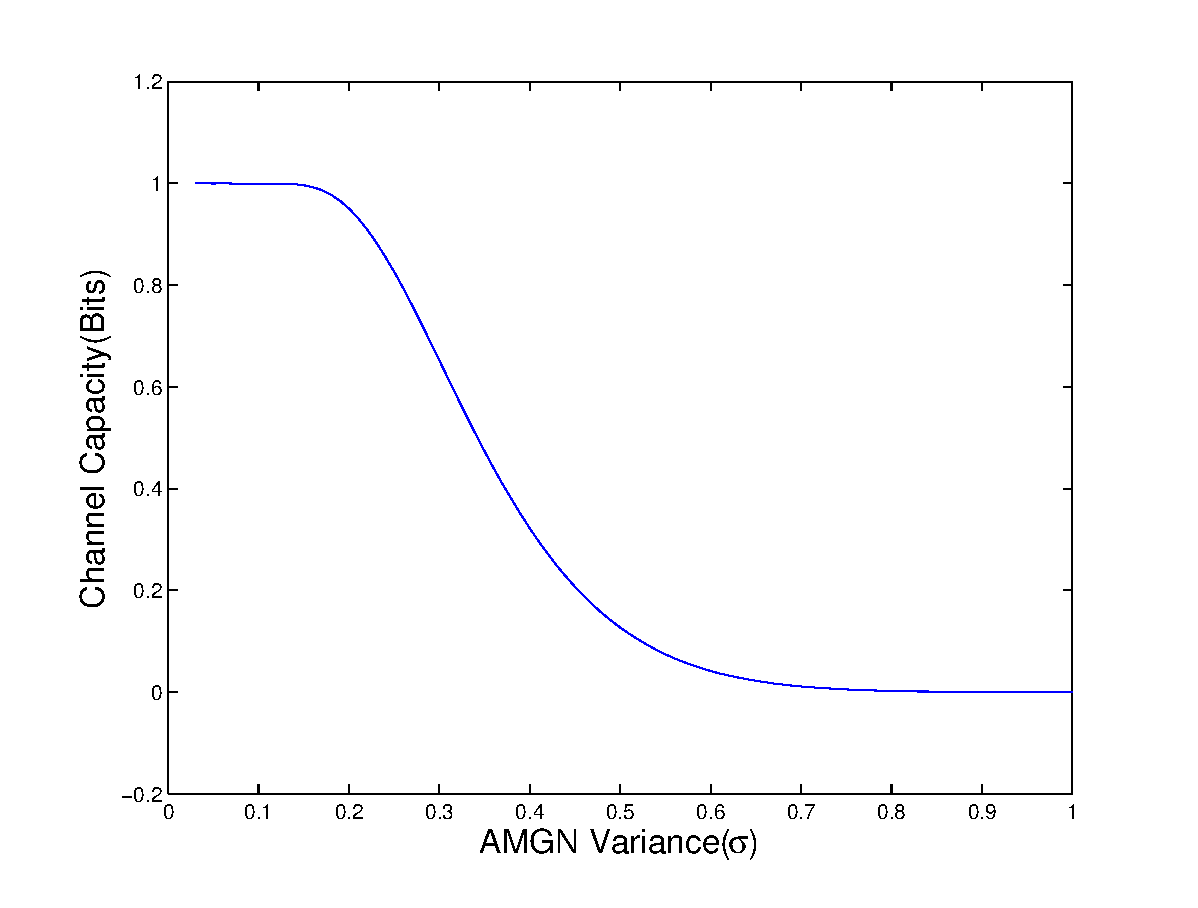
\includegraphics[width=4in]{./figures/Cap_integer_coset_lattice.eps}
%\caption{Channel capacity of the AMGN channel}
%\label{AMGNCapacity}
%\end{figure}

Let the number of levels required be $r+1$, with $r$ levels using nested CU-SC-LDPC codes and the last level be the $\Z_{2^r}^{n}$ uncoded lattice. The effective noise seen by $i^{\text{th}}$ level is denoted as $\sigma_{i}\defeq\sigma/2^{i-1}$. For $n=2 \times 10^{5}$, $r=2$ and target block error probability of $10^{-4}$, the target bit error probability in the uncoded level $P(\Z,\sigma_{r+1}^{2})$ is $5 \times 10^{-10}$. This corresponds to a $\sigma_{r+1}= 0.0804$. For this standard deviation, the equivalent capacities of the mod-$\Lmb$ channel at each level are given by $C(\Z/2\Z,\sigma_{r})=0.9923$,
$C(\Z/2\Z,\sigma_{r-1})=0.5726$ and $C(\Z/2\Z,\sigma_{r-2})=0.0242$. Observe that the capacity for level $r-2$ is almost zero which renders coding for this level unnecessary although this results in a very small increase in VNR (due to rate the loss) of $0.145$dB $(=20\log_{10}2^{0.0242})$. We use $r=2$ (i.e., 3 levels) and ($14,3,30$) CU-SC-LDPC ensemble with $L=32, w=4$ is used for the first two levels and the uncoded $\Z_{4}^{n}$ lattice is used in the last level.
\begin{table}
\centering
\caption{DE thresholds and Gap from Poltyrev limits (without rate loss from termination) for SC-LDPC lattice ensembles for various degree profiles.}
\begin{tabular}{c c c c c c c}
\hline  \hline
$(d_{c},d_{v}^{1},d_{v}^{2})$ &(L,w)& $P(\Z_{4},\sigma^{2})$ & $\sigma_{\text{max}}$ &$\text{VNR}$ &$\text{VNR}_{\text{rate-loss}}$\\
\hline
(60, 42, 3)& (80, 16)& $1 \times 10^{-6}$ & 0.4020 & 0.106dB &0.952dB\\
(60, 26, 3)& (72, 12)& $5 \times 10^{-10}$ & 0.3200 &0.482dB & 0.927dB\\
(60, 27, 3)& (64, 9)& $5 \times 10^{-10}$  &  0.3203 & 0.57dB & 0.951dB\\
(30,14,3) & (32,4) & $5 \times 10^{-10}$ & 0.3184 & 1.02dB & 1.347dB
\end{tabular}
\label{Table:Thresholds}
\end{table}
Due to the symmetry in the lattice, the all-zero lattice point is assumed to be transmitted. Instead of plotting the symbol error rate, we focus on determining the thresholds of the resulting lattice under BP decoding. We estimate the BP threshold from simulations by determining the maximum noise variance $\sigma_{\text{max}}^{2}$ for which no codeword errors are observed, at each coded level,  in simulation of 10 consecutive codewords each of length $2\times 10^{5}$.
%We calculate the maximum standard deviation $\sigma_{\text{max}}$ for which both levels of the lattice can be decoded. $\sigma_{\text{max}}=\min(\sigma_{1}^{\text{BP}},2\sigma_{2}^{\text{BP}})$, where $\sigma_{1}^{\text{BP}}$ and $\sigma_{2}^{\text{BP}}$ are the respective BP thresholds for the two SC-LDPC codes.
The VNR threshold is then calculated for the given rates and $\sigma_{\text{max}}$. The VNR estimated from the BP threshold is $1.14$dB ($1.46$dB with rate loss due to termination) whereas the estimate from the DE threshold for this ensemble is given by  $1.02$dB. We observe that the BP thresholds are very close to DE thresholds.
%
%Thus obtained BP thresholds $\sigma_{1}^{\text{BP}}$, $\sigma_{2}^{\text{BP}}$ for the above codes are $0.3142$ and $0.2161$ respectively which results in a VNR of $1.14$dB ($1.46$dB with rate loss due to termination). The DE predicted values are $0.3184$ and $0.21836$. We observe that the BP thresholds are very close to DE thresholds. i.e., the parameters are large enough to assume that the BP thresholds can be approximated by DE thresholds.
%
For a few other SC-LDPC ensembles, Table. \ref{Table:Thresholds} shows the noise threshold computed using DE and the corresponding VNR. Note that the Poltyrev limit is zero dB. The gap to the Poltyrev limit is primarily due to the fact that there is a mismatch between the rates that are obtainable for the proposed ensemble with a fixed $d_c$ and the capacity of the equivalent channel.
%
%very high capacity ($\approx 1$) in the last level and a very low capacity ($\approx 0$) in the first level and there is a mismatch in the rate of the LDPC code and the corresponding capacity. Even though SC-LDPC codes of such extreme rates (requires complex degree profiles) can be implemented thus achieving the Poltyrev limit, BP decoding for such high degrees becomes computationally complex.

This gap can be substantially decreased if the target bit error probability of $10^{-6}$ is used instead of a block error probability of $10^{-4}$. In this case, the capacities of the channels at each level are $0.9507, 0.3223$ and $0.0024$. The pair of nested codes from the (42,3,60) CU-SC-LDPC ensemble have rates 0.95 and 0.3 and match very closely the channel capacities (negligible rate loss). This reduces the gap to 0.106~dB and this is reported in the last row in the table.

\section{Application - Interference Channels}
%\subsection{Problem Statement}
We consider the 3 user Gaussian IC consisting of 3 transmitters, 3 receivers, and 3 independent messages originally considered in \cite{sridharan2008capacity}, where message $W_{j}$ originates at transmitter $j$ and is intended for receiver $j$, $\forall j\in \mc{J}\defeq\{1,2,3\}$. The output observed at the receiver $j$ is given by
\begin{align}\label{SymmInterfChannel}
    \mathbf{y}_{j}=\mathbf{x}_{j}+ \sum^{3}_{k=1,k\neq j}h_{jk}\mathbf{x}_{k}+\mathbf{z}_{j}, \hspace{10pt} \forall j\in \mc{J}
\end{align}
where $\mathbf{x}_{j}$ is the transmitted signal at $j^{\text{th}}$ transmitter, $h_{jk}$ are the channel parameters for the cross links, and $\mathbf{z}_{j}\sim\mc{N}(\mathbf{0},\sigma^{2}\cdot \mathbf{I})$ is the AWGN noise. If the channel parameters for all the cross links are equal to $\beta$, we refer to such model as a symmetric IC. The channel input signals are subjected to the power constraint
$\frac{1}{n}\sum_{i=1}^{n}E\left[\|\mathbf{x}_{j}\|^2\right]\leq P$.

%For a $2$-user symmetric Gaussian interference channel (IC) it was shown in \cite{carleial1978interference} that, in the very strong interference regime, the capacity region for the IC is as if there is no interference at all. For this symmetric model, a simple extension of the very strong interference condition for the 2 user IC %\cite{carleial1978interference}
%to the 3 user one is given by \cite{sridharan2008capacity}
%\begin{align}
%\beta^{2}\geq \frac{\left((1+P)^{2}-1\right)\left(1+P\right)}{2P}.
%\label{Eqn:StrongInterfCondition1}
%\end{align}

Sridharan \textit{et al.} in \cite{sridharan2008capacity} introduce a scheme where each user uses a lattice code and each receiver first decodes the total interference (aligned due to lattice structure) observed and then decodes the desired message. For this case, based on lattice decoding, they showed that interference can be decoded first if
\begin{align}
\beta^{2}(\sigma)\geq \beta^{*^{2}}(\sigma)\defeq\frac{(P+\sigma^{2})^{2}}{P\sigma^{2}}.
\label{Eqn:StrongInterfCondition2}
\end{align}
in which case, each user can achieve a rate of $\frac{1}{2}\log(1+\frac{P}{\sigma^{2}})$.
%If \eqref{Eqn:StrongInterfCondition2} is satisfied, each user can achieve a capacity \cite{sridharan2008capacity} of
%$\frac{1}{2}\log(1+\frac{P}{\sigma^{2}})$. Equivalently, for a given rate $R$, maximum noise variance under which the rate can be achieved is given by
%\begin{align}
%\sigma^{2}_{\text{max}}=\frac{P}{2^{2R}-1}.
%\label{Eqn:SigmaShannon}
%\end{align}
\subsection{Applying the Proposed Lattices}
Encouraged by the Poltyrev-limit achieving property of the proposed lattice ensembles under BP decoding, we use SC-LDPC lattice codes for the symmetric Gaussian IC in the very strong interference region. We will consider the case of using $r=2$ levels in the multistage code for ease of exposition, but the idea naturally extends to more levels. Let $\Lmb$ be the SC-LDPC lattice defined in \eqref{Eqn:ConstrD} with $r=2$.
% and a code from $(30,15,5)$ CU-SC-LDPC ensemble is used for the two levels.
We define the SC-LDPC lattice code $\mc{C}_{SCL}$ based on $\Lmb$ using hypercube shaping:
\begin{align}
\mc{C}_{SCL}=\left\lbrace \mathbf{\boldsymbol\lambda} \mod \Z_{4}^{n}: \mathbf{\boldsymbol\lambda} \in \Lmb \right\rbrace
\end{align}
where $n$ is the dimension of $\Lmb$. Let codeword $\mathbf{c}_{j}\in\mc{C}_{SCL}$ at transmitter $j$ be
\begin{align}
%\mathbf{c}_{j}&= \sum_{i=1}^{k_{1}}\alpha_{1i}^{j}\mathbf{g}_i+2\sum_{i=1}^{k_{2}}\alpha_{2i}^{j}\mathbf{g}_i \mod \Z_{4}^{n}\hspace{15pt} \alpha_{1i}^{j},\alpha_{2i}^{j}\in \{0,1\}\\
\label{Eqn:SICCodeword}
&= \sum_{i=1}^{k_{1}}\alpha_{1i}^{(j)}\mathbf{g}_i\!+\! 2\sum_{i=1}^{k_{2}}\alpha_{2i}^{(j)}\mathbf{g}_i\! -\! 4\mathbf{k}_{j}, \hspace{10pt} \alpha_{1i}^{(j)},\alpha_{2i}^{(j)}\! \in \{0,1\}
\end{align}
where ``$+$" denotes addition in $\R^{n}$ and $\mathbf{k}_{j}\in\Z^{n}$. Each codeword $\mathbf{c}_{j}\in\mc{C}_{SCL}\subset\{0,1,2,3\}^{n}$ is modulated to $\mathbf{\tilde{x}}_{j}\defeq \mathbf{c}_{j}-1.5^{n}$ such that $\mathbf{\tilde{x}}_{j}\in\mc{A}\defeq\{-1.5,-0.5,+0.5,+1.5\}^{n}$. At transmitter $j$, a dither vector $\mathbf{d}_{j}$ uniformly distributed among $\mc{B}\defeq [-2,2)$ is added to obtain the transmitted signal $\mathbf{x}_j$ given by
\begin{align}
\mathbf{x}_{j}=\mathbf{\tilde{x}}_{j}+\mathbf{d}_{j} \mod \Z_{4}^{n},
\label{Eqn:SICdither}
\end{align}
where the mod operation is over $\mc{B}$ instead of $[0,4)$. The dither vector achieves the purpose of randomizing the interference and helps in treating the undesired components of the received signal as additive uncorrelated noise. It can be seen that $\mathbf{x}_{j}$ is uniformly distributed over $\mc{B}$ and the average power of the transmitted signal at each transmitter is $1.33$.
\subsection{Decoding}
%Before looking at the general case
Let us consider the case of symmetric Gaussian IC i.e $h_{12}=h_{13}=\beta$ and without loss of generality consider receiver 1. 
%The system flow from the perspective of receiver 1 is given in Fig.~\ref{Fig:SIC_decoder}.
%\begin{figure}[h!]
%\centering
%%\begin{document}
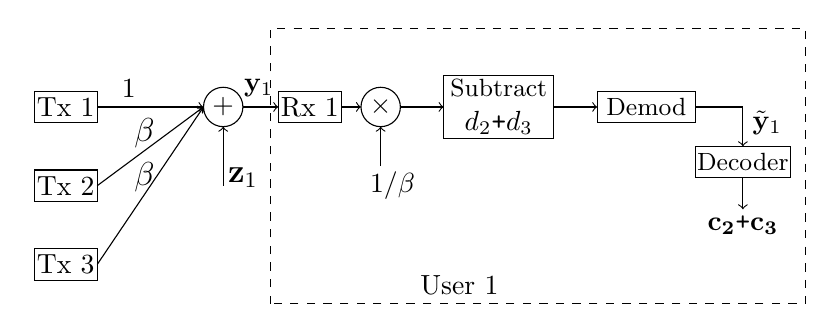
\begin{tikzpicture}

%3 Users
\draw[black] (0.4,0.2) rectangle (-0.4,-0.2); \node at (0,0) {\normalsize Tx 1};
\draw[black] (0.4,-0.8) rectangle (-0.4,-1.2); \node at (0,-1) {\normalsize Tx 2};
\draw[black] (0.4,-1.8) rectangle (-0.4,-2.2); \node at (0,-2) {\normalsize Tx 3};

%Oblique lines to Plus block
\draw [->] (0.4,0) -- (1.75,0); \node [above] at (0.8,0) {1};
\draw [->] (0.4,-1) -- (1.75,0); \node [above] at (1,-0.65) {\large $\beta$};
\draw [->] (0.4,-2) -- (1.75,0); \node [above] at (1,-1.2) {\large $\beta$};


%From + end to Rx1 end
\draw[black] (2,0) circle (0.25); \node at (2,0) {+};
\draw [->] (2,-1) -- (2,-0.25);\node at (2.25,-0.9) {\large $\mathbf{z}_{1}$};

%Receiver 1 block
\draw[black] (2.7,-0.2) rectangle (3.5,0.2); \node at (3.1,0) {\normalsize Rx 1};
\draw [->] (2.25,0) -- (2.7,0);\node[above] at (2.45,0) {\normalsize $\mathbf{y}_{1}$};

%From Rx1 end to 1/beta multiplicator end
\draw[black] (4,0) circle (0.25); \node at (4,0) {$\times$};
\draw [->] (4,-0.75) -- (4,-0.25);\node at (4.15,-1) {\normalsize $1/\beta$};
\draw [->] (3.5,0) -- (3.75,0);

\draw[black] (4.8,0.4) rectangle (6.2,-0.4) node[pos=0.5,align=center] {\small Subtract\\ $d_{2}\texttt{+}d_{3}$}; 
%\node[text width=1.2,align=left] at (5.05,0) {\normalsize Subtract  \\ $d_{2}\texttt{+}d_{3}$};
\draw [->] (4.25,0) -- (4.8,0);

% Input to the Demod
\draw[black] (6.75,0.2) rectangle (8,-0.2) node[pos=0.5,align=center] {\small Demod};
\draw [->] (6.2,0) -- (6.75,0);

%Input to Decoder
\draw [->](8,0) -- (8.6,0) -- (8.6,-0.5);
\node[right] at (8.6,-0.2) {\normalsize $\tilde{\mathbf{y}}_{1}$};
\draw[black] (8,-0.9) rectangle (9.2,-0.5) node[pos=0.5,align=center]  {\small Decoder}; 

%Overview dashed rectangle
\draw [->] (8.6,-0.9) -- (8.6,-1.3);  \node at (8.6,-1.5){\normalsize $\mathbf{c_{2}}\texttt{+}\mathbf{c_{3}}$};
\draw [dashed] (2.6,-2.5) rectangle (9.4,1);\node [above] at (5,-2.5) {\normalsize User 1};

 \end{tikzpicture}
%\end{document} 
%\caption{System flow for the 3-user symmetric Gaussian interference channel at receiver 1.}
%\label{Fig:SIC_decoder}
%\end{figure}
The input to the multistage decoder at receiver 1 is given by
\begin{align*}
\tilde{\mathbf{y}}_{1} &\defeq \frac{\mathbf{y}_{1}}{\beta}-\mathbf{d}_{2}-\mathbf{d}_{3}+1.5^{n}+1.5^{n}\\%\mod \Z_{4}^{n} \\
&=\mathbf{c}_{2}+\mathbf{c}_{3}+\frac{1}{\beta}\left(\mathbf{x}_{1}+\mathbf{z}_{1}\right).
\end{align*}
The key here is that $\mathbf{c}_{2},\mathbf{c}_{3}\in\mc{C}_{SCL}\subset\Lmb$ and hence $\mathbf{c}_{2}+\mathbf{c}_{3}\in \Lmb$ is given by
\begin{align*}
%&	 \mathbf{c}_{2}\!+\!\mathbf{c}_{3}&=\\
&\sum_{i=1}^{k_{1}}\left(\alpha_{1i}^{(2)}\!+\!\alpha_{1i}^{(3)}\right)\mathbf{g}_i\!+\!2\sum_{i=1}^{k_{2}}\left(\alpha_{2i}^{(2)}\!+\!\alpha_{2i}^{(3)}\right)\mathbf{g}_i +4(\mathbf{k}_{2}+\mathbf{k}_{3})\\
=&\sum_{i=1}^{k_{1}}\left(\alpha_{1i}^{(2)}\!\oplus\!\alpha_{1i}^{(3)}\right)\mathbf{g}_i+2\sum_{i=1}^{k_{2}}\left(c_{1i}\oplus\alpha_{2i}^{(2)}\oplus\alpha_{2i}^{(3)}\right)\mathbf{g}_i +4\mathbf{k}_{23}
\end{align*}
where $c_{1i}=0.5\left(\alpha_{1i}^{(2)}+\alpha_{1i}^{(3)}-\alpha_{1i}^{(2)}\oplus\alpha_{1i}^{(3)}\right)$, $c_{2i}=0.5\left(c_{1i}+\alpha_{2i}^{(2)}+\alpha_{2i}^{(3)}-c_{1i}\oplus\alpha_{2i}^{(2)}\oplus\alpha_{2i}^{(3)}\right)$ are carryovers from first and second levels respectively and
 $\mathbf{k}_{23}=\mathbf{k}_{2}+\mathbf{k}_{3}+\sum_{1}^{k_{2}}c_{2i}\mathbf{g}_{i}\in\Z^{n}$. Since $c_{1i}, c_{2i} \in \{0,1\}$, using the multistage decoder described in Section \ref{Sec:SCLDPC}, one can directly decode the lattice point $\mathbf{x}_{2}+\mathbf{x}_{3}$(interference), subtract it and decode the desired signal.
The decoding scheme above extends to the case when one channel gain is an integer multiple of the other, but this is not shown here.

%For example, let $h_{13}=Kh_{12}$
%where $K=\sum_{0}^{l-1}a_{i}2^{i}\in \Z, a_{i}\in\{0,1\}$. In this case, input to the multi-stage decoder is
%%where $K=\sum_{0}^{l-1}a_{i}2^{i}\in \Z$, $a_{i}\in\{0,1\}$. In this case input to the multi-stage decoder is
%\begin{align*}
%\tilde{\mathbf{y}}_{1} &\defeq \frac{\mathbf{y}_{1}}{h_{12}}-\mathbf{d}_{2}-K\mathbf{d}_{3}+1.5^{n}+K1.5^{n}\\
%&=\mathbf{c}_{2}+K\mathbf{c}_{3}+\frac{1}{h_{12}}\left(\mathbf{x}_{1}+\mathbf{z}_{1}\right).
%\end{align*}
%where $\mathbf{c}_{2}+K\mathbf{c}_{3}$ is a lattice point and is given by
%\begin{align*}
%%\mathbf{c}_{2}+K\mathbf{c}_{3}=
%\sum_{i=1}^{k_{1}}\left(\alpha_{2i}\oplus a_{0}\alpha_{3i}\right)\mathbf{g}_i+2\sum_{i=1}^{k_{2}}\left(c_{1i}\oplus\beta_{2i}\oplus a_{0}\beta_{3i}\oplus a_{1}\alpha_{3}\right)\mathbf{g}_i+4\mathbf{k}
%\end{align*}
%for some $\mathbf{k}\in\Z^{n}$.



\subsection{Simulation Results for Symmetric IC}
We first present simulation results for successful decoding of the interference. For the $(18,3,30)$ ensemble with $r=2$, we fixed $\sigma = 0.3728$ and increased $\beta$ until we were able to successfully decode the interference. The value of $\beta^2$ for which the interference could be decoded was within $0.396$~dB from the limit in  \eqref{Eqn:StrongInterfCondition2} showing that proposed scheme is able to operate very close to the theoretical limits. We now present results on decoding the desired user. For these results, we assume that the interference has been successfully decoded. In Fig.~\ref{Fig:ShapingLoss} we plot the achievable rate (sum-capacity of a 4-level Construction-D lattice code) as a function of $P/\sigma^2$ for the desired user for $r=4$ and compare it to the corresponding Shannon limit.  The DE thresholds with the proposed SC-LDPC codes is also shown in the plot and it can be seen that the DE thresholds are very close to the achievable rates. It can be seen that the DE threshold is roughly 2.559dB away from the Shannon limit at high rates, of which 1.53dB  can be explained with loss due to hypercube shaping. The SNR required to successfully decode 10 consecutive codewords from simulations are also shown as BP thresholds. Simulation results are shown for four cases - (i) $r=4$, 3.41 bits/channel use, $(26,3,3,3,60)$ CU-SC-LDPC ensemble, (ii) $r=4$, 3.26 bits/channel use, $(35,3,3,3,60)$ CU-SC-LDPC ensemble, (iii) $r=3$, 2.46 bits/channel use, $(26,3,3,60)$ CU-SC-LDPC ensemble, (iv) $r=3$, 2.21 bits/channel use, $(35,3,3,60)$ CU-SC-LDPC ensemble. In all these cases, $(L,w)=(72,12)$ was used.% and we ignored the rate loss due to termination.



%and we analyze the bit error probability in decoding the interference versus the channel gain $\beta$. We observe that within $0.396$dB of the very strong interference regime given by \eqref{Eqn:StrongInterfCondition2} we are able to decode the interference with a bit error probability of less than $10^{-6}$. Note that the main bottle neck in error performance in decoding the interference is the last i.e., the uncoded level whereas in decoding the desired signal (after the interference is decoded and subtracted), within $\sigma_{\text{max}}$, arbitrarily small error rates can be achieved since no uncoded level needs to be decoded.

%On a single user AWGN channel i.e, after the interference is subtracted, the DE threshold for this code for the given parameters is computed to be $\sigma_{\text{max}}=0.3351$ whereas asymptotically the maximum achievable variance is $\sigma_{\text{AMGN}}=0.3728$. The Shannon capacity from \eqref{Eqn:SigmaShannon} is given by $\sigma_{\text{Sh}}=0.4969$ which is equivalent to a gap of $2.5$dB.

%We also observe that as the number of levels increase this gap converges to $1.53$dB which corresponds to the loss due to the sub-optimal hypercube shaping. For a 4-level binary lattice code with hypercube shaping corresponding gap between shannon capacity and the sum-capacity of 4 levels is plotted  in Fig. \ref{Fig:ShapingLoss}. One can also observe that the sum-capacity can be very closely achieved with a SC-LDPC lattice code of maximum check node degree 60.
%Thus we claim that with optimal shaping strategies the capacity of the $K$-user symmetric Gaussian IC \cite{sridharan2008capacity} in the very strong interference channel can be achieved.

\begin{figure}
\centering
\setlength\figureheight{4.5cm}
\setlength\figurewidth{7cm}
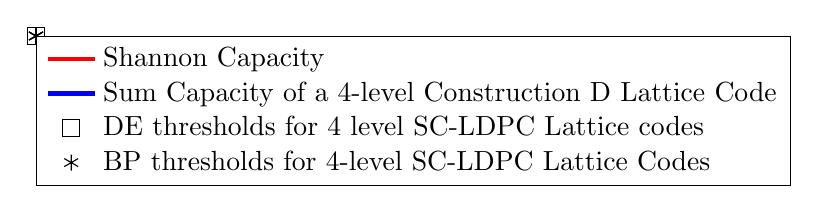
\begin{tikzpicture}
\def\fsize{\normalsize}
\begin{axis}[
width=\figurewidth,
height=\figureheight,
scale only axis,
xmin=4,
xmax=30,
xlabel={$\text{P/}\sigma{}^{\text{2}}\text{dB}$},
ymin=0,
ymax=5,
legend style={at={(0,1)},anchor=north west,draw=black,fill=white,legend cell align=left}
]
\addplot [color=red,solid,line width=1.5pt]
table[row sep=crcr]{
1 0.587818317346194\\
3 0.791341177455778\\
5 1.0286866043034\\
7 1.29390718678102\\
9 1.58040221195651\\
11 1.88219718352143\\
13 2.19452948368152\\
15 2.51390383667526\\
17 2.83788995090244\\
19 3.16485622972095\\
21 3.49373172947796\\
23 3.8238235812452\\
25 4.1546876206064\\
27 4.48604077166048\\
29 4.81770328916082\\
31 5.14956130632863\\
33 5.48154279616551\\
35 5.81360224010802\\
};
\addlegendentry{Shannon Capacity};

\addplot [color=blue,solid,line width=2.0pt]
table[row sep=crcr]{
1 0.108452421861326\\
3 0.30023434461803\\
5 0.583744051972549\\
7 0.908016893863155\\
9 1.23986729393466\\
11 1.57212348172311\\
13 1.90441001540582\\
15 2.23669080702334\\
17 2.56895109146972\\
19 2.90120263165125\\
21 3.23173038940203\\
23 3.54445589072375\\
25 3.7941222586385\\
27 3.93912155348957\\
29 3.99069691963094\\
31 3.99949543839257\\
33 3.99999469407798\\
35 3.99999999597798\\
};
\addlegendentry{Sum Capacity of a 4-level Construction D Lattice Code};

\addplot [color=black,mark size=3.0pt,only marks,mark=square,mark options={solid}]
table[row sep=crcr]{
21.4693 3.15\\ % 18.91 3.1501 
22.3844 3.2667\\  %19.621 3.2668 . The commented out values are the snr values at which the shannon capacity is equal
23.1876 3.4167\\  %20.532 3.4166 	   to the DE of the optimal degree profiles of the 4 level SCLDPC lattice code.
15.4486951388326 2.2\\
16.3638449500461 2.3167\\
17.1669877129645 2.4667\\
};
\addlegendentry{DE thresholds for 4 level SC-LDPC Lattice codes};

\addplot [color=black,mark size=2.9pt,only marks,mark=asterisk,mark options={solid}]
table[row sep=crcr]{
23.2798476914952 3.41666666666667\\
22.4669998480458 3.26666666666667\\
16.3950035382421 2.31666666666667\\
17.2078513816915 2.46666666666667\\
};
\addlegendentry{BP thresholds for 4-level SC-LDPC Lattice Codes};


\draw[<->] (axis cs:18.91,3.1501 ) -- (axis cs:21.469, 3.15);
\draw[->] (axis cs:19.6,3.12) to [out=285,in=175] (axis cs:22,2.6);
%\node[font=\scriptsize] at (axis cs:14,3.6){1.57dB};
\node[font=\fsize] at (axis cs:24,2.6){2.559dB};

	\end{axis}
\end{tikzpicture}%
\caption{Achievable rates for the desired user assuming the interference has been decoded.}	
\label{Fig:ShapingLoss}	
\end{figure}

\bibliographystyle{ieeetr}
\bibliography{journal_abbr,bib_SCLDPC}

\end{document} 